\FloatBarrier
\section{Exploratory input-derivative measurements}
\label{app:input}
A separate grid contains 28 models: four methods at three reference seeds, plus four methods at seed 0 under each of four changes (learning rate $0.0025$ or $0.01$, weight decay $10^{-4}$ or $2\times10^{-3}$). All use CIFAR-10 (50k training / 10k test images), ResNet-20-BN/ReLU, SGD and 30 epochs. These twenty method--recipe conditions are exploratory; the changed recipes have only one seed and are not recommended hyperparameters. All diagnostics concern final checkpoints.

\subsection{Input Jacobians and finite logit changes}
Let $x\in[0,1]^{3\times32\times32}$ be an image in raw intensity units. Per-channel normalization is included inside $f_\theta(x)\in\R^{10}$, the vector of logits. With the model in eval mode, saved BatchNorm statistics and the final intervention state, we compute
\[
 J(x)=\frac{\partial f_\theta(x)}{\partial x}\in\R^{10\times3072}.
\]
Ten backward passes give the rows of $J$; singular values follow from its float64 $10\times10$ Gram matrix. Norms average the first 1,000 images in the pinned training order, without class balancing. Units are logits per unit input intensity. Logit scaling can change these norms without changing classification decisions; they do not give the uniform bounds required by a margin argument such as \citet{sokolic2017robust}.
% GENERATED by paper/tools/build_assets.py from data/records/ -- do not edit by hand.
% Regenerate: py paper/tools/build_records.py && py paper/tools/build_assets.py
\begin{table}[!t]
\caption{Input diagnostics in the separate reference grid: CIFAR-10 / ResNet-20-BN / SGD, 30 epochs, saved BatchNorm; mean $\pm$ sample SD over three seeds. Jacobian norms average 1k training images and use raw-intensity coordinates. Radius is in cycles per image. Bold accuracy means exceed Plain.}\label{tab:input-reference}
\centering\small\setlength{\tabcolsep}{4pt}\renewcommand{\arraystretch}{1.08}
\begin{tabular*}{\linewidth}{@{\extracolsep{\fill}}lrrrr@{}}
\toprule
Method & \multicolumn{1}{c}{Test accuracy (\%)} & \multicolumn{1}{c}{$\mathbb E\|J\|_F$} & \multicolumn{1}{c}{$\mathbb E\|J\|_2$} & \multicolumn{1}{c}{Mean radius}\\
\midrule
Plain & $75.93\pm1.04$ & $143.2\pm1.8$ & $78.7\pm2.3$ & $12.08\pm0.33$\\
Resolution & $\mathbf{80.22}\pm0.01$ & $100.0\pm3.6$ & $53.6\pm2.0$ & $12.63\pm0.17$\\
Gaussian & $\mathbf{79.95}\pm0.04$ & $74.8\pm4.0$ & $39.5\pm2.2$ & $11.01\pm0.25$\\
Combined & $\mathbf{81.35}\pm0.09$ & $78.1\pm1.4$ & $41.6\pm0.8$ & $11.46\pm0.18$\\
\bottomrule
\end{tabular*}
\end{table}


For the spatial Fourier profile, we apply an orthonormal two-dimensional transform to each Jacobian row, sum squared magnitudes over logits and channels, and group them by rounded radius. Energy fractions are normalized within each 250-image batch, then averaged over four batches. The energy-weighted mean radius is in cycles per image; this is a batch-normalized Jacobian spectrum, not a mean of per-image normalized spectra.

For each image, let $v_1(x)$ be a unit top right singular vector of $J(x)$. The finite input diagnostic is
\[
 D(\varepsilon)=\frac1N\sum_i
 \|f_\theta(x_i+\varepsilon v_1(x_i))-f_\theta(x_i)\|_2,
 \quad \varepsilon\in\{0.05,0.1,0.25,0.5,1,2,3,6,12\}.
\]
The singular direction is fixed at the original image. Inputs are not clipped to $[0,1]$, so large perturbations leave the image domain. This logit displacement differs from the CE sensitivity $S$. At $\varepsilon=0.5$, the ratio $D(\varepsilon)/(\varepsilon\,\mathbb E\sigma_{\max}(J))$ is about 0.32--0.47 in the reference runs: the local linear approximation is already inadequate.

\begin{figure}[htbp]\centering
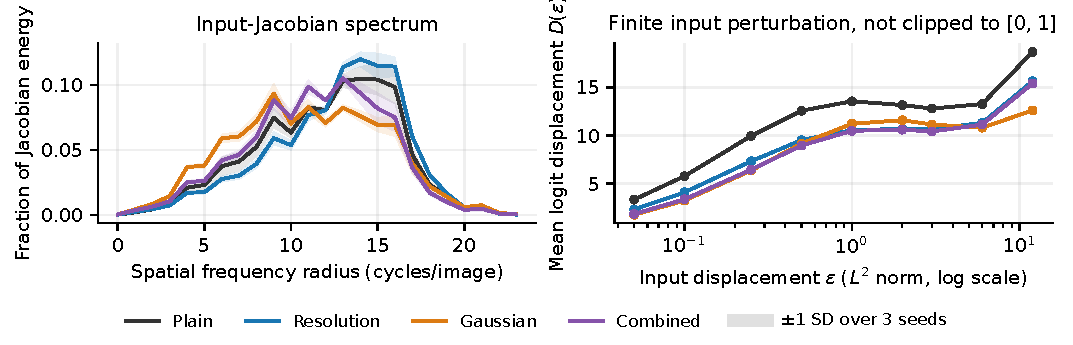
\includegraphics[width=.90\linewidth]{figures/input_diagnostics.pdf}
\caption{Input-diagnostic reference group. Left: Jacobian frequency profiles, mean $\pm$ SD over three seeds. Right: mean logit displacement along the top input singular direction, without clipping. R lowers the Jacobian norm but increases its mean frequency radius.}
\label{fig:input}
\end{figure}
All three interventions lower the mean Jacobian norms, but R increases the mean frequency radius whereas G and RG decrease it (Table~\ref{tab:input-reference}). These measurements therefore do not establish a common low-frequency explanation of improved accuracy.

\subsection{Parameter trace and cross-condition analysis}
The grid also estimates the Hessian trace of mean training CE on 5,000 images, with saved BatchNorm and all 269,722 parameters, including biases and normalization parameters. Five power-iteration components deflate a 64-draw Rademacher Hutchinson estimate \citep{hutchinson1989trace}. Mean reference traces are $\tJacPlainTrace$ (Plain), $\tJacRTrace$ (R), $\tJacGTrace$ (G) and $\tJacRGTrace$ (RG). The parameter subset, data and solver differ from Appendix~\ref{app:hessian-checks}, so the two studies are not pooled.

Of \tGridEstimates{} power-iteration estimates, \tGridConverged{} met a relative-change threshold of $10^{-4}$ within 40 iterations, including all \tGridCells{} leading estimates. This is not an eigenvector-residual certificate; the main Hessian comparison uses the residual-checked Lanczos results.

Table~\ref{tab:input-grid} gives the full twenty-condition grid. Exploratory correlations with test error, controlling training error, weakened when restricted to intervention conditions. Unequal replication, few conditions and joint dependence on method and recipe limit that analysis. It neither validates a predictor on held-out conditions nor establishes causality.


% GENERATED by paper/tools/build_assets.py from data/records/ -- do not edit by hand.
% Regenerate: py paper/tools/build_records.py && py paper/tools/build_assets.py
\begin{table}[!htbp]
\caption{All twenty input-diagnostic conditions: CIFAR-10 / ResNet-20-BN / SGD, 30 epochs. Each block changes one reference hyperparameter. Entries are means over $n$ seeds; changed recipes have one seed and no estimated SD. CE uses the full training/test sets; Jacobian norms use 1k training images. The all-parameter trace uses 5k images. Bold accuracy means exceed Plain within the same recipe.}\label{tab:input-grid}
\centering\small\setlength{\tabcolsep}{4pt}\renewcommand{\arraystretch}{1.08}
\begin{tabular*}{\linewidth}{@{\extracolsep{\fill}}lrrrrrr@{}}
\toprule
Method & \multicolumn{1}{c}{$n$} & \multicolumn{1}{c}{Test acc. (\%)} & \multicolumn{1}{c}{Train CE} & \multicolumn{1}{c}{Test CE} & \multicolumn{1}{c}{$\mathbb E\|J\|_F$} & \multicolumn{1}{c}{$\widehat{\mathrm{tr}}(H)$}\\
\midrule
\addlinespace[4pt]\multicolumn{7}{@{}l@{}}{\textit{Reference: $\eta=0.005$, $w=5\times10^{-4}$}}\\[2pt]
Plain & 3 & $75.93$ & $0.209$ & $0.755$ & $143.2$ & $14\,731$\\
Resolution & 3 & $\mathbf{80.22}$ & $0.300$ & $0.577$ & $100.0$ & $10\,108$\\
Gaussian & 3 & $\mathbf{79.95}$ & $0.270$ & $0.595$ & $74.8$ & $10\,361$\\
Combined & 3 & $\mathbf{81.35}$ & $0.311$ & $0.552$ & $78.1$ & $8\,761$\\
\addlinespace[4pt]\multicolumn{7}{@{}l@{}}{\textit{Learning rate $\eta=0.0025$}}\\[2pt]
Plain & 1 & $71.33$ & $0.600$ & $0.816$ & $83.7$ & $12\,308$\\
Resolution & 1 & $\mathbf{74.08}$ & $0.606$ & $0.741$ & $69.9$ & $9\,863$\\
Gaussian & 1 & $\mathbf{75.52}$ & $0.507$ & $0.706$ & $60.0$ & $11\,541$\\
Combined & 1 & $\mathbf{76.76}$ & $0.533$ & $0.668$ & $63.8$ & $9\,473$\\
\addlinespace[4pt]\multicolumn{7}{@{}l@{}}{\textit{Learning rate $\eta=0.01$}}\\[2pt]
Plain & 1 & $78.21$ & $0.024$ & $0.790$ & $189.3$ & $4\,744$\\
Resolution & 1 & $\mathbf{82.95}$ & $0.092$ & $0.546$ & $135.6$ & $7\,356$\\
Gaussian & 1 & $\mathbf{81.93}$ & $0.124$ & $0.563$ & $81.6$ & $7\,245$\\
Combined & 1 & $\mathbf{83.88}$ & $0.158$ & $0.487$ & $100.1$ & $6\,525$\\
\addlinespace[4pt]\multicolumn{7}{@{}l@{}}{\textit{Weight decay $w=10^{-4}$}}\\[2pt]
Plain & 1 & $73.58$ & $0.256$ & $0.793$ & $147.6$ & $12\,536$\\
Resolution & 1 & $\mathbf{80.03}$ & $0.332$ & $0.590$ & $102.6$ & $8\,701$\\
Gaussian & 1 & $\mathbf{79.54}$ & $0.310$ & $0.607$ & $73.5$ & $9\,243$\\
Combined & 1 & $\mathbf{80.72}$ & $0.343$ & $0.568$ & $79.3$ & $7\,534$\\
\addlinespace[4pt]\multicolumn{7}{@{}l@{}}{\textit{Weight decay $w=2\times10^{-3}$}}\\[2pt]
Plain & 1 & $77.23$ & $0.146$ & $0.697$ & $132.2$ & $22\,648$\\
Resolution & 1 & $\mathbf{81.94}$ & $0.213$ & $0.537$ & $91.2$ & $17\,584$\\
Gaussian & 1 & $\mathbf{81.91}$ & $0.197$ & $0.535$ & $63.2$ & $16\,493$\\
Combined & 1 & $\mathbf{83.18}$ & $0.233$ & $0.489$ & $72.0$ & $14\,604$\\
\bottomrule
\end{tabular*}
\end{table}


\paragraph{Validation and scope.}
All 28 re-evaluated test accuracies match their training-log endpoints, with CE discrepancies below $2\times10^{-8}$ nats. The intervention runs have unusually narrow seed spreads (R: $80.21,80.22,80.22\%$). Initial-weight and data-order records distinguish the seeds, and trajectories diverge, but final-checkpoint hashes were unavailable to the audit. We keep this batch separate and make no claim of reduced seed variance.
